\subsection{Laying pipes in the clouds}\label{sec:rate-control}

\begin{figure*}[!t]
  \centering
    \begin{subfigure}{0.65\columnwidth}
  \centering
  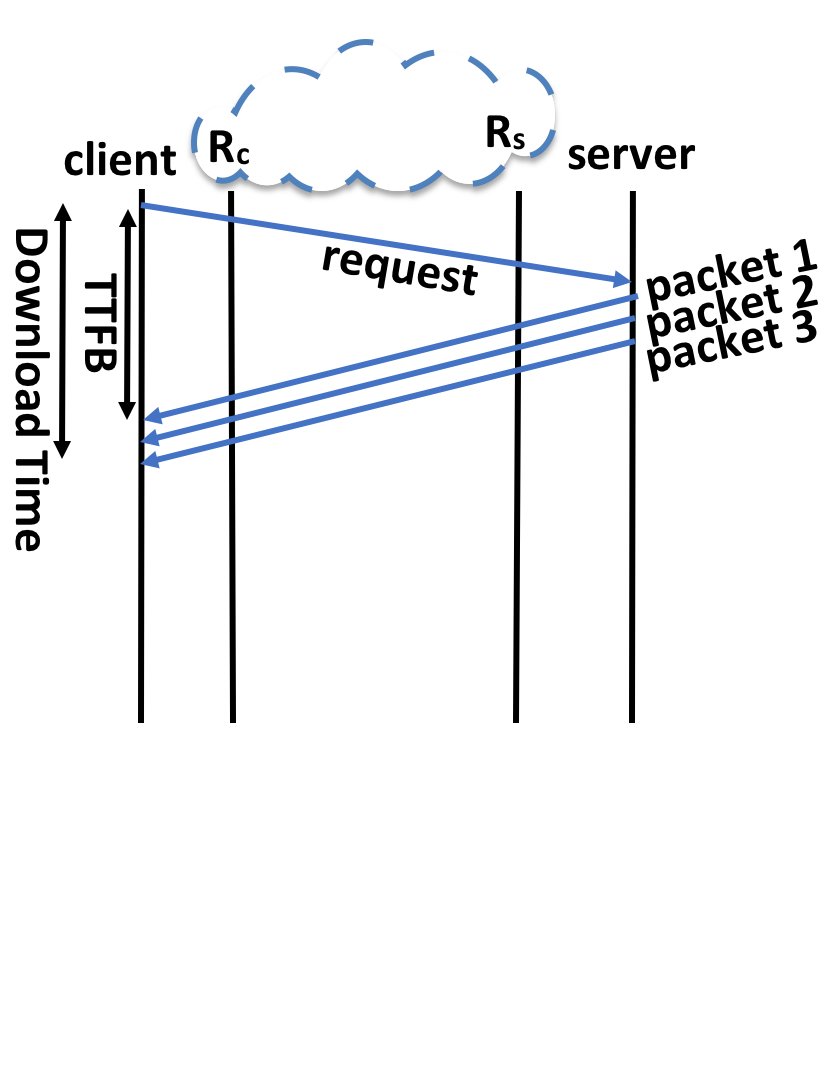
\includegraphics[width=\columnwidth]{figures/ideal.png}
    \caption{Ideal protocol-free transmission.}
    \label{fig:ideal}
\end{subfigure}    \quad
\begin{subfigure}{0.65\columnwidth}
  \centering
  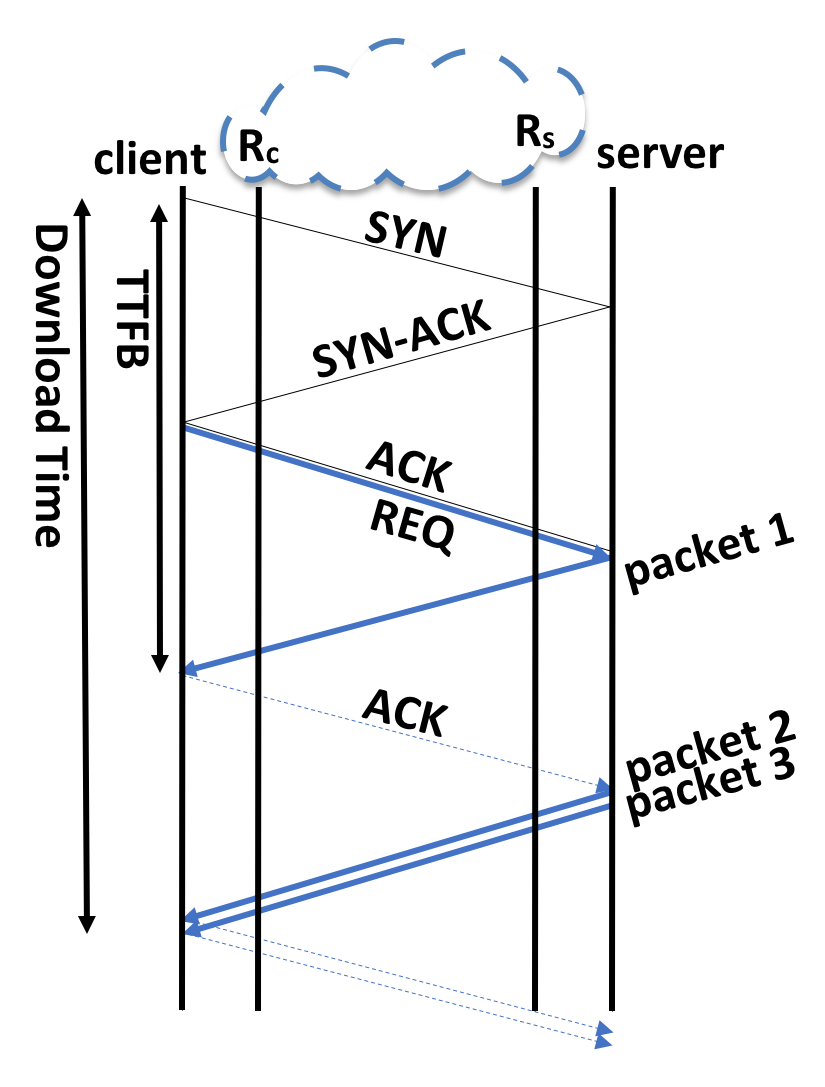
\includegraphics[width=\columnwidth]{figures/e2e.png}
    \caption{End-to-end (no split) transmission.} \label{fig:e2e}
\end{subfigure}    \quad
\begin{subfigure}{0.65\columnwidth}
  \centering
  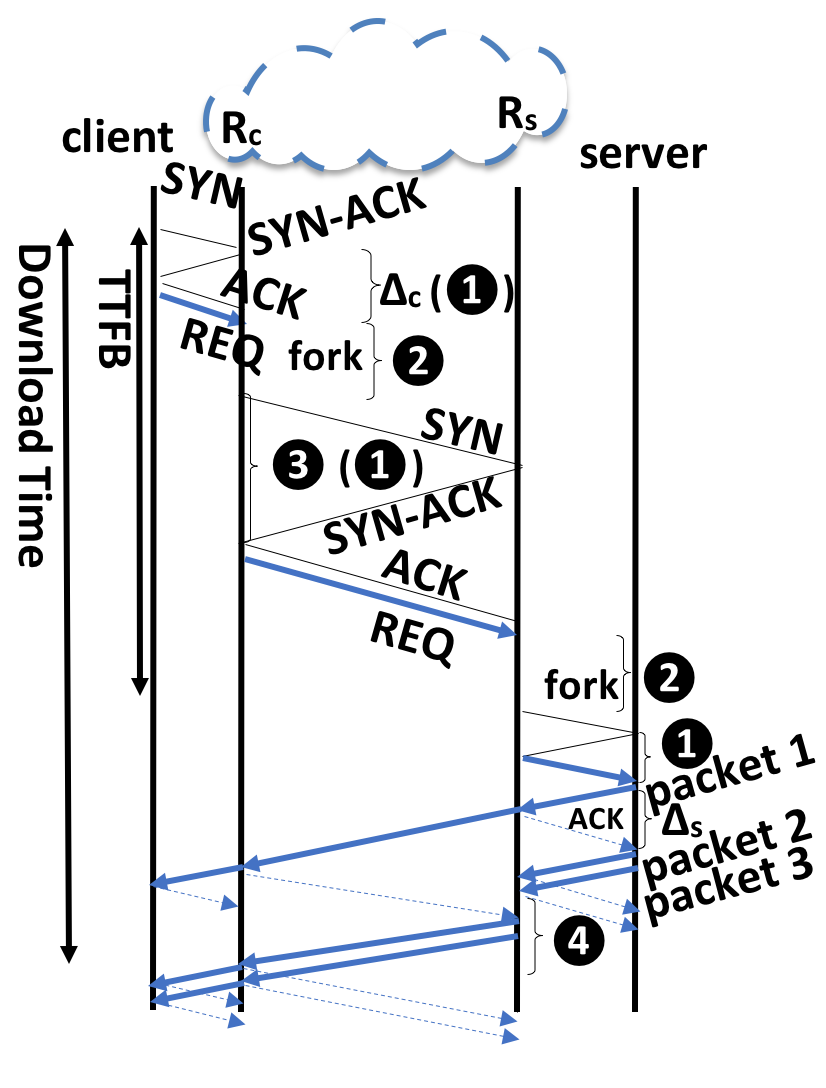
\includegraphics[width=\columnwidth,clip]{figures/split.png}
    \caption{Simple TCP split, on both \rc and \rs} 
    \label{fig:baseline}
\end{subfigure}

    \caption{Illustrated comparison of the considered baseline data transmission methods.}
\end{figure*}

\begin{figure*}[!t]
  \centering
    \begin{subfigure}{0.75\columnwidth}
  \centering
  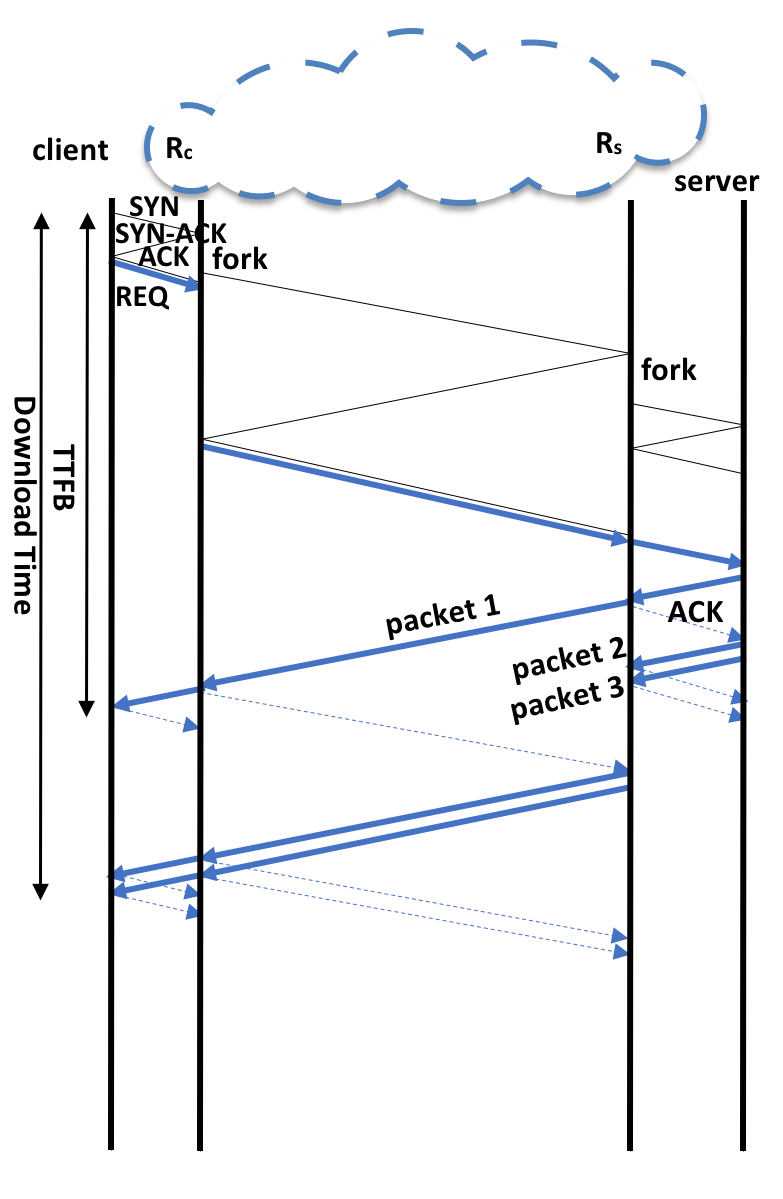
\includegraphics[width=\columnwidth]{figures/early-syn.png}
    \caption{Early-SYN.}
    \label{fig:early-syn}
\end{subfigure}    \hfill
\begin{subfigure}{0.75\columnwidth}
  \centering
  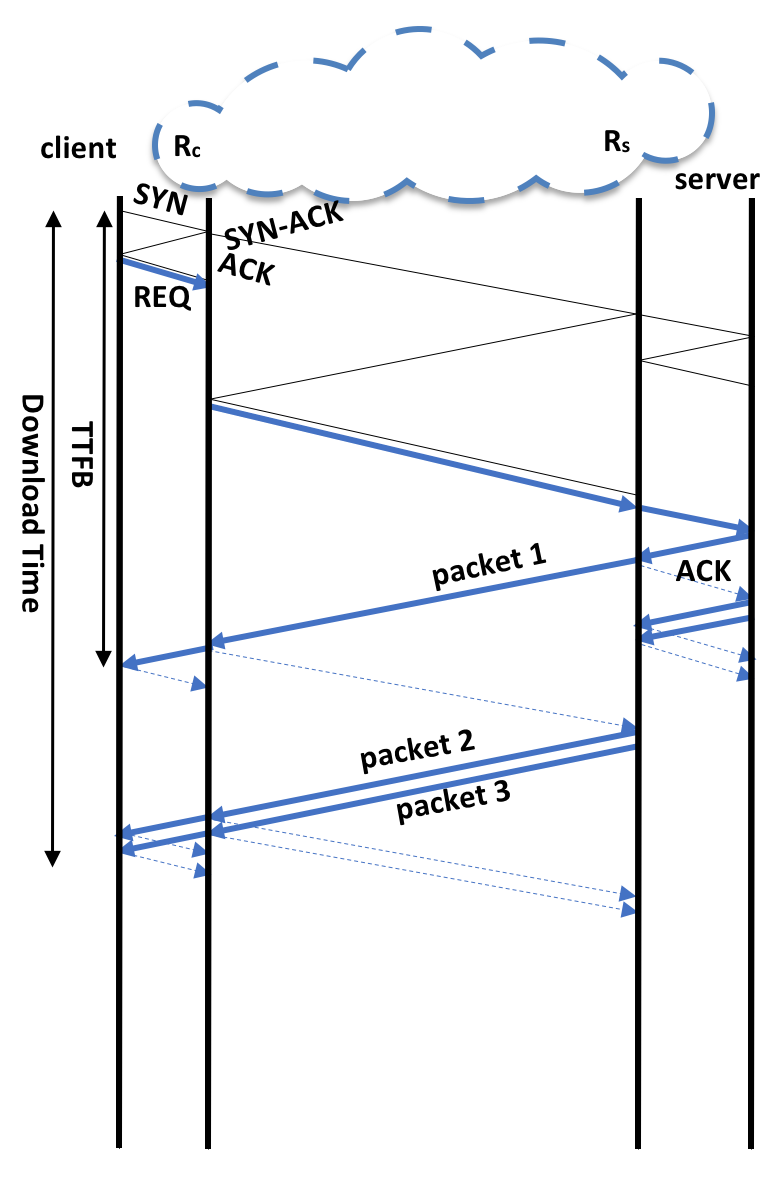
\includegraphics[width=\columnwidth]{figures/thread.png}
    \caption{Thread pool.} \label{fig:thread-pool}
\end{subfigure}    \centering
\begin{subfigure}{0.75\columnwidth}
  \centering
  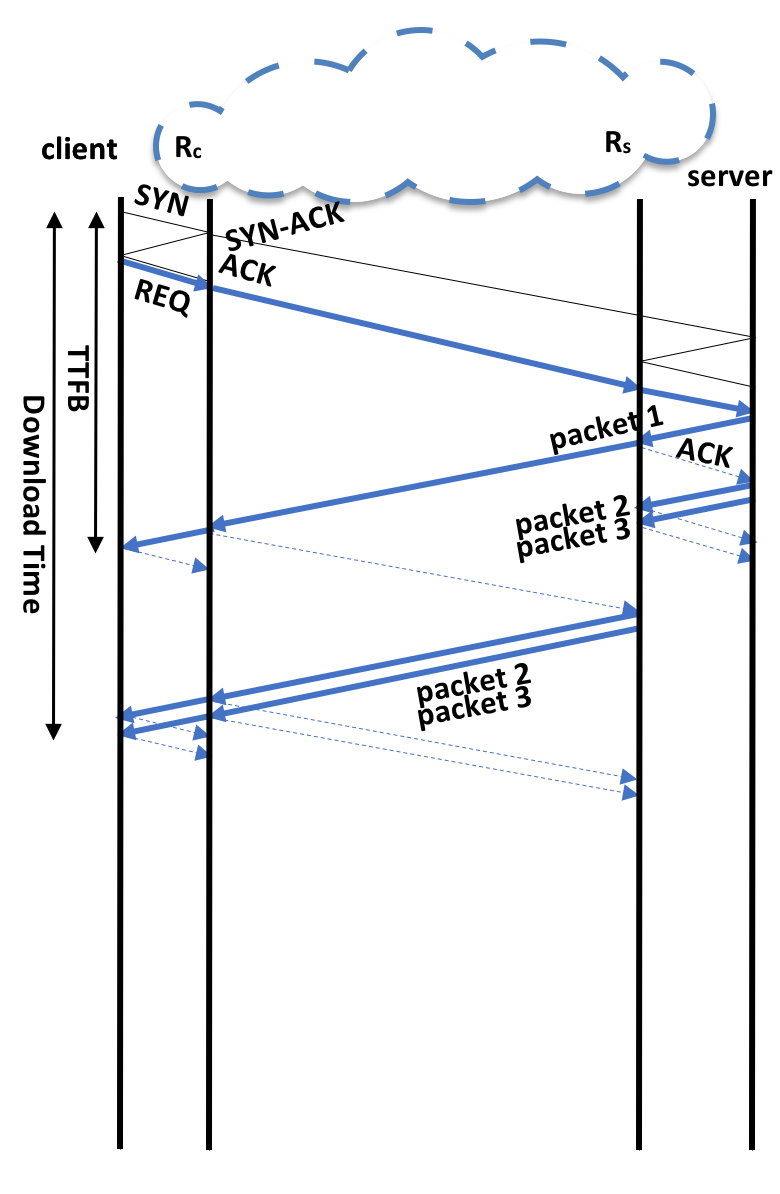
\includegraphics[width=\columnwidth]{figures/connection.png}
    \caption{Connection pool.} \label{fig:connection-pool}
\end{subfigure}     \hfill
\begin{subfigure}{0.75\columnwidth}
  \centering
  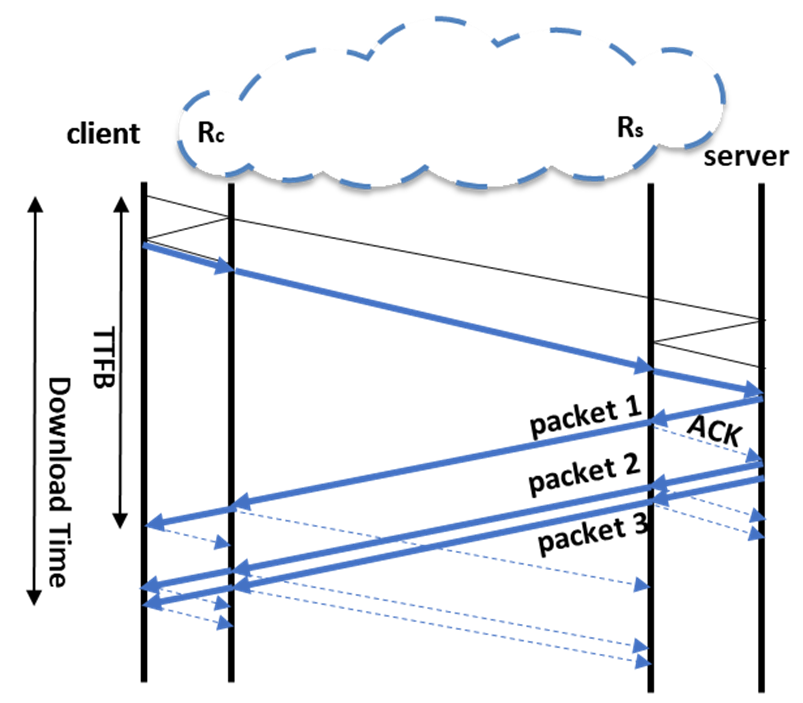
\includegraphics[width=\columnwidth]{figures/turbo.png}
    \caption{Turbo-Start TCP.} 
    \label{fig:turbo-start-tcp}
\end{subfigure}

    \caption{\oursys successive implementation improvements}
    \label{fig:oursys-improvements}
\end{figure*}

%\begin{figure}[t]
%  \centering
%\begin{subfigure}{0.7\columnwidth}
%  \centering
%  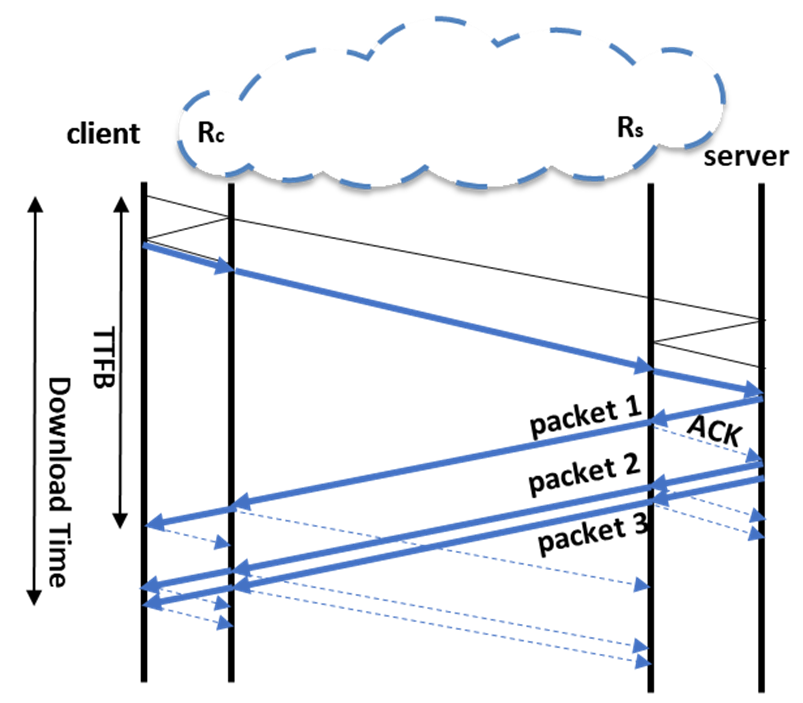
\includegraphics[width=\columnwidth]{figures/turbo.png}
%    \caption{Turbo-Start TCP.} \label{fig:turbo-start-tcp}
%\end{subfigure}
%
%    \caption{Illustrated comparison of the considered baseline data transmission methods.}
%\end{figure}

%\T{Congestion-less control?} The cloud provides an auto-scaling networking infrastructure with links of virtually-infinite capacity. Like others~\cite{haq2017measuring}, we find that in-cloud paths provide more predictable results than the public Internet, with an order of magnitude lower loss rate. As a result, flows in the cloud will rarely ever encounter congestion. This compels us to rethink the role of congestion control in the cloud. In light of the near-absence of congestion, we essentially want a simple high-rate sending protocol capable of dealing with the very rare loss events, without necessarily backing off. Even flow control is not necessarily needed within the cloud, as clouds can increasingly provide an elastic memory infrastructure~\cite{hotadd,baloon} that can quickly adapt to any receive-buffer temporary load. 

%\T{Ideal pipe.} 
The cloud provides an auto-scaling networking infrastructure with links of virtually-infinite capacity. As a result, flows in the cloud will rarely ever encounter congestion. Like others~\cite{haq2017measuring}, we find that in-cloud paths provide more predictable results than the public Internet, with an order of magnitude lower loss rate. Given the favorable conditions in the cloud, we wonder if we could facilitate an ideal transmission. \autoref{fig:ideal} illustrates our fundamental model of an ideal transmission. Importantly, this model reflects a protocol-free, theoretical and ideal transmission; thus we are free to disregard overheads like the TCP three way handshake.\\
 \textit{Ideal (\autoref{fig:ideal}):} In an ideal scenario, we would like to wait no more than one round-trip time (RTT), for the response to our request to start arriving. In this case the request would go through the \relays directly triggering the transmission of all response packets. The time-to-first-byte (TTFB) would be just one RTT, the lowest possible TTFB.\\
Unfortunately, the classical end-to-end data transfer shown in \autoref{fig:e2e}, falls short of this ideal model. In this example, we suppose that the client requests three MSS-sized packets using HTTP over TCP, that the initial TCP window size is one MSS, and that there are no losses.\\
 \textit{Real (\autoref{fig:e2e}):} End-to-end\footnote{Iin this case the \relays just forward packets, without any additional logic} HTTP transmission over TCP, first requires the establishment of an end-to-end connection, adding one RTT to the ideal finish time. Waiting one RTT for the first ACK further delays the download.\\
 %\AB{Did you mean the ACK sent from the client on the first data packet from the server, and that this is due to TCP's cwnd behavior? It wasn't clear when I read this.}.\\ 
Now, when we add additional logic to the \relays, in addition to the delays caused by TCP, more delays are added. These delays are shown in \autoref{fig:baseline}.\\
\textit{TCP Split (\autoref{fig:baseline}): } The basic TCP split mechanism, divides the long control loop into several separate legs, each with a shorter control loop. This separation, results in shorter download time for larger files. But a naive implementation also introduces additional overheads. Due to these overheads TCP split may be detrimental for small file downloads. The main overheads stem from: (1) on demand resource allocation on the VM, and (2) socket semantics, that result in the legs of the connections being established successively .In section ~\ref{sec:approx} we discuss TCP split overheads in greater detail.  We can address the delays marked (1)-(4) in \autoref{fig:baseline}, but we are left with delays $\Delta_c$ and $\Delta_s$ on the client and server sides, respectively. The best way to shorten these $\Delta$, is by decreasing the RTT(\ie physical distance) to their respective \relays. 

\section{Approximating the Ideal Pipe}\label{sec:approx}

To approximate the ideal data transmission model, we introduce \textit{\oursys}.
The goal of \oursys is to provide efficient, delay-free TCP optimization while utilizing commodity VMs and standard programming APIs. We introduce four improvements over the naive TCP split approach. The effects of these improvements are illustrated in Figure~\ref{fig:oursys-improvements}. 

%.  . Turbo-Start TCP eliminates delay (4). The two last delays (marked as ``?'' in Figure~\ref{fig:baseline}) that need be removed are delays $\Delta_c$ and $\Delta_s$ on the client and server sides, respectively. As both depend on the client and server parameters, are beyond our control.

%\oursys incorporates four improvements to the baseline strategy of Section~\ref{x}, illustrated in Figure~\ref{fig:baseline}. Together, these four improvements eliminate the delays marked (1)-(4) in \ref{fig:oursys-improvements}. We next elaborate on each of the four improvements. We discuss the many implementation details involved in realizing \oursys in Section~\ref{sec:design}.

\T{Improvement 1: Early SYN.} \xspace Figure ~\ref{fig:early-syn}. In early SYN~\cite{ladiwala,siracusano2016miniproxy}, a SYN packet is sent to the next-hop server as soon as the SYN packet arrives. This is done without waiting for the three-way handshake to complete. \oursys captures this first SYN packet and triggers the start of a new connection. This allows the proxy to establish the two legs of a split connection in parallel. Using \textit{Early-SYN}, we can remove SYN-ACK and ACK delays, marked as (1) in Figure~\ref{fig:baseline}.
While the notion of creating the two legs of the connection in parallel is not new, ours is the first to use standard Linux utilities.

\T{Improvement 2: Thread pool.}     \xspace Figure ~\ref{fig:thread-pool}.
The creation of new processes or threads for each new split connection is \\time-consuming and adds greatly to the connection jitter. Some outliers may take tens of milliseconds, greatly hurting performance. For small files/objects, this jitter may even nullify the benefit of \oursys. To mitigate this problem, we create a pool of reusable threads. These are sleeping threads, awaiting to accept new tasks. Using a \textit{thread pool} removes the delays marked as (2) in Figure ~\ref{fig:baseline}. 

\T{Improvement 3: Reusable connections.} \xspace Figure ~\ref{fig:connection-pool}. This optimization aims to improve the performance of long-haul connections, \ie those where the RTT between the two cloud relays dominates. The goal is to negate the delay of the long three-way handshake. We achieve this goal by preemptively connecting to distant \relays. On each \relay we create a pool of \reconn between each pair of distant \relays.
With a \textit{connection pool}, delay (3) in Figure~\ref{fig:baseline} is eliminated.

\T{Improvement 4: Turbo-Start TCP.} \xspace Figure ~\ref{fig:turbo-start-tcp}.
Congestion is not an issue within the cloud, hence, there is essentially no need to use TCP's slow-start mechanism. It is redundant to probe the network when a connection is established between two \relays within the same cloud provider. We thus configure a large initial congestion window (CWND) and large receive window (RWIN). In addition, we increase the socket buffers for the relay machines, so that memory would not limit the performance of the intra-cloud flows.
Note that we do not change the CWND used on any Internet-facing flows. We wish to remain friendly to other TCP flows potentially sharing a bottleneck link with our \relays.

%\subsection{Rate-Control Within the Cloud}
%Turbo-start TCP\AB{To be completed}

%\subsection{Congestion Control at the Edge}


%\subsection{Putting it all together: We are close to Pipe}

